\chapter{\label{chap:konzeption}Konzeption}
Die erarbeiteten Anforderungen zur Untersuchung der Konfliktmanagementstrategien offlinefähiger Systeme werden in diesem Kapitel für die Konzeption angewendet.\\
Es soll für jede zu untersuchende Technologie ein Prototyp entwickelt werden. Im Rahmen dieser Arbeit entsteht ein Prototyp der \sc{Redux Offline} verwendet und ein zweiter in dem \sc{PouchDB} und \sc{CouchDB} eingesetzt wird. Für letzteren könnte genausogut \sc{Hoodie} als Framework benutzt werden, da es sowohl PouchDB als auch CouchDB benutzt~\cite{hoodie-how}, doch da für den zu entwickelnden Prototyp lediglich diese beiden Komponenten benötigt werden, wurde sich dagegen entschieden.
\todo{Entscheidung Redux- Offline begründen?} Bis zu einem gewissen Status, nämlich dem der Verweindung der Technologien, sind beide Prototypen -- bis auf den Namen-- identisch.\\
Beginnend mit dem Aufbau der exemplarischen Anwendung werden in den folgenden Abschnitten die  Architektur  und schließlich \todo{blabla} aufgeführt.\\\\
Von den Namen der beiden Prototypen können die beinhalten verwendeten Technologien abgelesen werden. Der Prototyp der \sc{Redux Offline} verwendet heißt \it{amilia-rdx}. \it{amilia-qouch} benutzt PouchDB für die lokale Datenpeicherung im Browser und CouchDB als Serverdatenbank.
% Den Raum aller möglichen Lösungen anhand der Anforderungen auf die in irgendeinem Sinn beste / geeignetste einzuschränken:\\
% App entwickeln, in der es einen `Verbindung unterbrechen` Knopf gibt ', oder ob es aus irgendwelchen Erwägungen notwendig sein könnte, das über eine separate Instanz zu machen.
%
% Aufbau
%
\section{Anwendungsaufbau}
Die Prototypen bestehen im Frontend aus React und wurden mit \sc{Create React App}\footnote{\url{https://github.com/facebook/create-react-app}} erstellt. \sc{Create React App} erstellt ein Projekt mit dem gewünschten Namen, generiert eine initiale Projektstruktur (vgl. Abbildung \ref{fig:init}) und installiert die dafür benötigten Abhängigkeiten. Diese sind im Verzeichnis node\_modules installiert.
Außerdem ist ein ServiceWorker und ein App Manifest (\tt{manifest.json}) enthalten, wodurch die \gls{PWA}-- Kriterien erfüllt sind.\\
Als Template gibt es nun die \tt{public/index.html}-- Datei. In der \tt{index.js}--Datei werden die React--Komponenten und der ServiceWorker initialisiert.. Alle \tt{App.*}--Dateien umfassen eine minimale Beispielanwendung.
In der generierten \tt{package.json}--Datei (vgl. Abbildung \ref{fig:init2}), befinden sich Informationen über die Anwendung und ihre Abhängigkeiten. Im Unterpunkt \tt{scripts} werden Kommandozeilen-Aufrufe definiert und können mit dem Befehl \tt{npm} aufgerufen werden.
\begin{figure}[H]
  \centering
  \begin{subfigure}[t]{0.45\textwidth}
          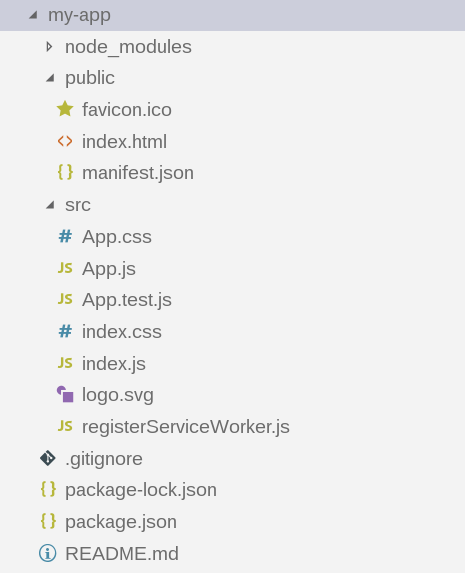
\includegraphics[width=\textwidth]{Ordnerstruktur}
          \caption{Die initiale Projektstruktur}
          \label{fig:init}
  \end{subfigure}
  ~ 
  \begin{subfigure}[t]{0.45\textwidth}
          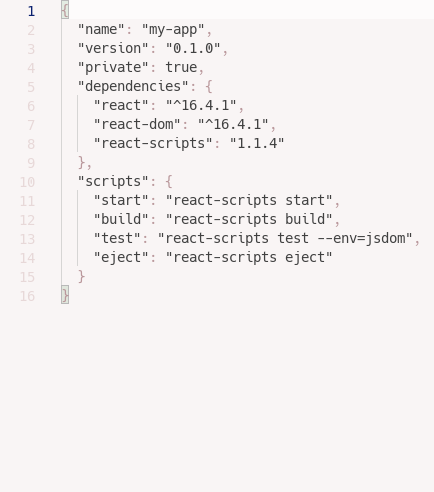
\includegraphics[width=\textwidth]{rca-package}
          \caption{Die initiale package.json Datei}
          \label{fig:init2}
  \end{subfigure}
  \grayRule
  \caption[Create React App: initiale Testapplikation]{einer mit Create React App erstellten Testapplikation}
  \label{fig:create-react-app}
\end{figure}
%
% React Komponenten
%
\sub{Aufbau der React Komponenten ?}
\todo{React und redux beschreiben?}
%
%
% Architektur
%
\section{Architektur}
Container\\
Header\\
Liste\\
Form\\
Konflikt--Dialog\\
\begin{figure}[H]
  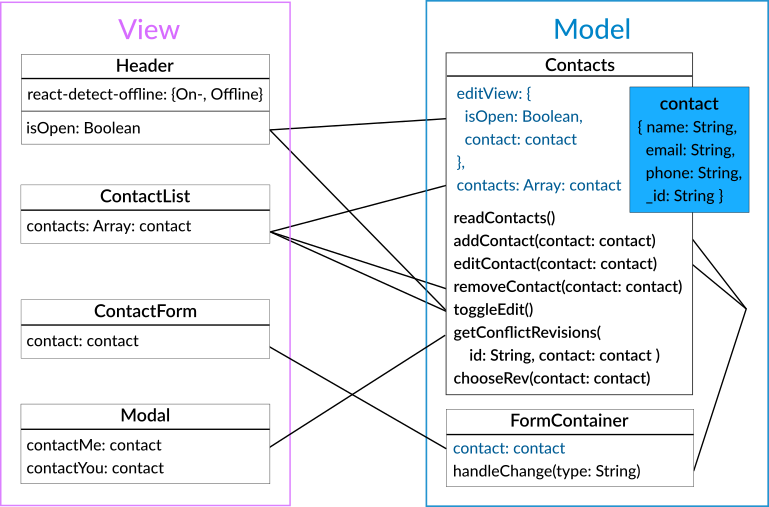
\includegraphics[width=\textwidth]{uml}
  \grayRule
  \caption{Komponentenarchitektur}
  \label{fig:uml}
\end{figure}
%
% Online / Offline
%
\sub{Verbindungsstatus feststellen}
React detect-offline
%
% Lokale Speicherung
%
\sub{Lokale Speichern der Daten}
% Redux Offline
\subsub{Lokale Speicherung mit Redux Offline}
Redux Offline: Idee: Store = Datenbank
% Pouch
\subsub{Lokale Speicherung mit PouchDB}
%
% Sync
%
\sub{Synchronisation}
% Redux Offline
\subsub{Synchronisation mit Redux Offline}
Redux Offline: Server der alle \gls{CRUD} Operationen unterstützt,
\gls{JSON}--Datei zur Persisierung um Ergebnisse nicht zu verfälschen 
Redux Offline: Idee: Store = Datenbank
% Pouch
\subsub{Synchronisation mit PouchDB}
CouchDB = RemoteDB\\
%
% UI
%
\section{Die graphische Oberfläche}
Aus den minimalen Anforderungen an die graphische Oberfläche ergibt sich das Design. Anhand der folgenden Abbildungen werden die gefertigten Entwürfe der BenutzerInnenoberfläche dargestellt.\\\\
Diese Listenansicht in Abbildung \ref{fig:list} besteht aus dem Header / Kopf und den Listeneinträgen. Sie zeigt die Kontakteinträge in beiden Netzwerkstatus: online (Abbildung \ref{fig:list-online}) und offline (\ref{fig:list-offline}).\\\\
Im Header ist abzulesen ob die Anwendung gerade eine Netzwerkverbindung hat oder nicht. Für eine bessere Prägnanz wurden hierzu unterstützend die Farben Rot für keine Verbindung und Grün für eine bestehende Netzwerkverbindung gewählt. Rechts im Header gibt es einen Knopf mit dem man in die Ansicht gelangt in der ein Kontakt hinzugefügt werden kann.\\
In der Liste sieht man die Namen der Person und jeweils einen Knopf zum Bearbeiten oder Löschen. Mit der Betätigung des `Delete`--Knopfs wird der entsprechende Eintrag in der Liste gelöscht
\begin{figure}[H]
  \centering
  \begin{subfigure}[t]{0.49\textwidth}
          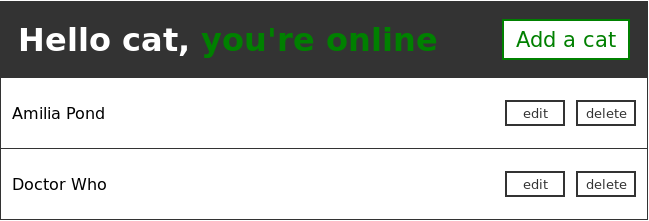
\includegraphics[width=\textwidth]{list-online}
          \caption{Kontaktliste im Onlinestatus}
          \label{fig:list-online}
  \end{subfigure}
  ~ 
  \begin{subfigure}[t]{0.49\textwidth}
          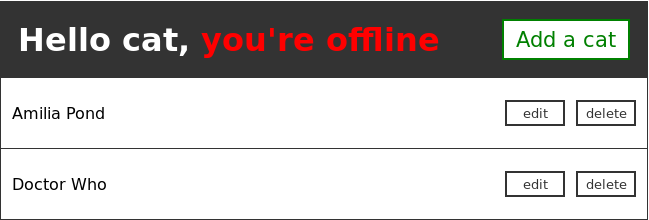
\includegraphics[width=\textwidth]{list-offline}
          \caption{Kontaktliste im Offlinestatus}
          \label{fig:list-offline}
  \end{subfigure}
  \grayRule
  \caption{Die Kontaktliste in beiden Netzwerkstatus}
  \label{fig:list}
\end{figure}
Klickt man auf den Knopf zum Bearbeiten oder auf den zum Hinzufügen eines Kontakts gelangt man in die Bearbeitungsansicht (vgl. Abbildung \ref{fig:edit}). Der Header ist bis auf den Knopf zum Hinzufügen eines Kontakts identisch zu dem der Liste. Auch hier ist abzulesen ob die Anwendung on-- oder offline ist. Da man sich bereits in der Ansicht zum Anlegen oder Editieren eines Kontaks befindet, ist der Knopf im Header überflüssig.\\
Ein Kontakt hat einen Namen, eine E-Mailadresse und eine Telefonnummer. In dieser Ansicht gibt es für jedes Attribut ein Eingabefeld. Die Felder sind beim Bearbeiten des Kontakts vorausgefüllt. Mittels Betätigung des `Speichern` Knopfs werden die Änderungen übernommen, klickt man auf `Cancel` werden sie verworfen. In beiden Fällen gelangt man wieder zur Listenansicht.
\begin{figure}[H]
  \centering
  \begin{subfigure}[t]{0.49\textwidth}
          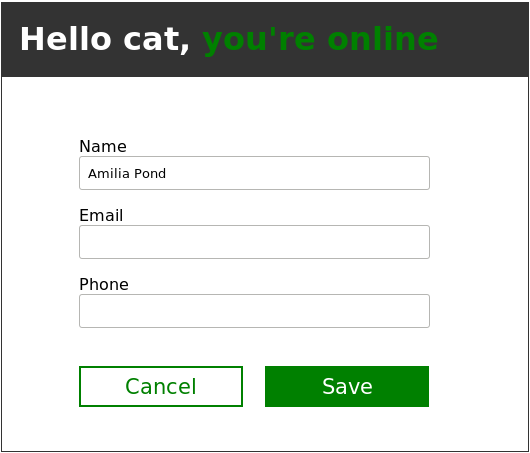
\includegraphics[width=\textwidth]{edit}
          \caption{Editieransicht im Onlinestatus}
          \label{fig:edit-online}
  \end{subfigure}
  ~ 
  \begin{subfigure}[t]{0.49\textwidth}
          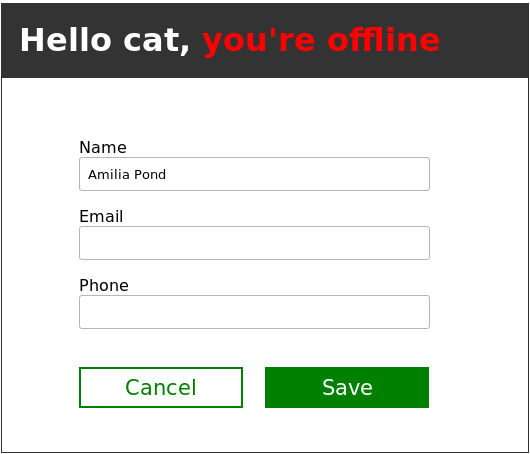
\includegraphics[width=\textwidth]{edit-offline}
          \caption{Editieransicht im Offlinestatus}
          \label{fig:edit-offline}
  \end{subfigure}
  \grayRule
  \caption{Die Editieransicht in beiden Netzwerkstatus}
  \label{fig:edit}
\end{figure}
\todo{Konfliktdialog}
%
% Testfälle
%
\section{Testfälle}
Folgende Testfälle werden während der Entwicklung stetig durchgeführt. Das erfolgreiche Bestehen dieser Tests ist eine notwendige Qualitätseigenschaft der zu entwickelnden Prototypen.
\begin{description}[leftmargin=0.7cm,style=nextline]
\item[Netzwerkstatus:] 
Die Anwendung muss zu jeder Zeit den korrekten Netzwerkstatus anzeigen.\\
\item[Kontakte lesen:] 
Die Anwendung bei jedem Start die Kontakte aus dem lokalen Speicher oder aus der \it{Datenbank} laden.\\
\item[Kontakt anlegen:] 
Die Anwendung muss zu jedem Zeitpunkt in der Lage sein einen Kontakt mit jedem seiner Attribute anzulegen. Dazu muss er immer lokal gespeichert werden und sobald eine Internetverbindung besteht, persistiert werden.
Das Anlegen eines Kontakts im Offlinestatus ist für die Konfliktforcierung erforderlich.\\
\item[Kontakt bearbeiten:] 
Die Anwendung muss zu jedem Zeitpunkt in der Lage sein einen Kontakt mit jedem seiner Attribute zu bearbeiten. Ist keine Internetverbindung vorhanden, müssen die Änderungen lokal übernommen und später, sobald sich der Netzwerkstatus ändert, synchronisiert werden.
Das Bearbeiten eines Kontakts im Offlinestatus ist für die Konfliktforcierung erforderlich.\\
\item[Kontakt löschen:] 
Die Anwendung muss zu jedem Zeitpunkt in der Lage sein einen Kontakt zu löschen.
Das Löschen eines Kontakts im Offlinestatus ist für die Konfliktforcierung erforderlich.\\
\end{description}